

\documentclass{beamer}

\mode<presentation> {


\usetheme{Madrid}



\setbeamertemplate{footline}[page number] 

\setbeamertemplate{navigation symbols}{} % To remove the navigation symbols from the bottom of all slides uncomment this line
}

\usepackage{graphicx} 


\usepackage{comment}
\usepackage{tikz}
\usepackage{booktabs} 
\usepackage{tikz-cd}
\usepackage{fontawesome}
\usepackage{apacite}
\renewcommand\bibliographytypesize{\footnotesize}
\usepackage{mathtools}
%\usepackage {tikz}
\usepackage{tkz-graph}
\GraphInit[vstyle = Shade]
\tikzset{
  LabelStyle/.style = { rectangle, rounded corners, draw,
                        minimum width = 2em, fill = yellow!50,
                        text = red, font = \bfseries },
  VertexStyle/.append style = { inner sep=5pt,
                                font = \normalsize\bfseries},
  EdgeStyle/.append style = {->, bend left} }
\usetikzlibrary {positioning}
%\usepackage {xcolor}
\definecolor {processblue}{cmyk}{0.96,0,0,0}

\title{SOM-where in Chicago} 

\author{Shakil Rafi \\ Ph.D. Candidate} 
\institute[University of Arkansas] 
{
University of Arkansas \\ 
\medskip
}
\date{\today} 

\begin{document}
\nocite{*}
\begin{frame}
\titlepage 
\end{frame}

\begin{frame}
\frametitle{Table of Contents} 
    \tableofcontents 
\end{frame}


\section{What is SOM}
\begin{frame}
\frametitle{Self-organizing maps, or Kohonen maps}
Self-organizing maps are neural networks architectures used for dimensionality reduction. \\
Proposed by Tuevo Kohonen in 1980, hence also called Kohonen maps.
\\
\end{frame}
\begin{frame}{The mathematical description}
	\begin{block}{The algorithm}
	initialize lattice nodes;\\
	initialize weight vectors; \\
	N $\leftarrow$ iteration count; \\
	\textbf{for} $i$ in $N$:	\\
	\quad	$x \leftarrow$ pick random point in dataset; \\
	\quad 	$c \leftarrow$ select lattice closest to $x$;\\
	\quad 	move weight vector of c closer to $x$;\\
	\quad 	move weight vectors of the neighbors of $c$ slightly closer to $x$
	\end{block}

\end{frame}
\begin{frame}{Lattice Architecture}
	Typically we initialize a lattice over the data as either square lattices or hexagonal lattices:
	\begin{center}
	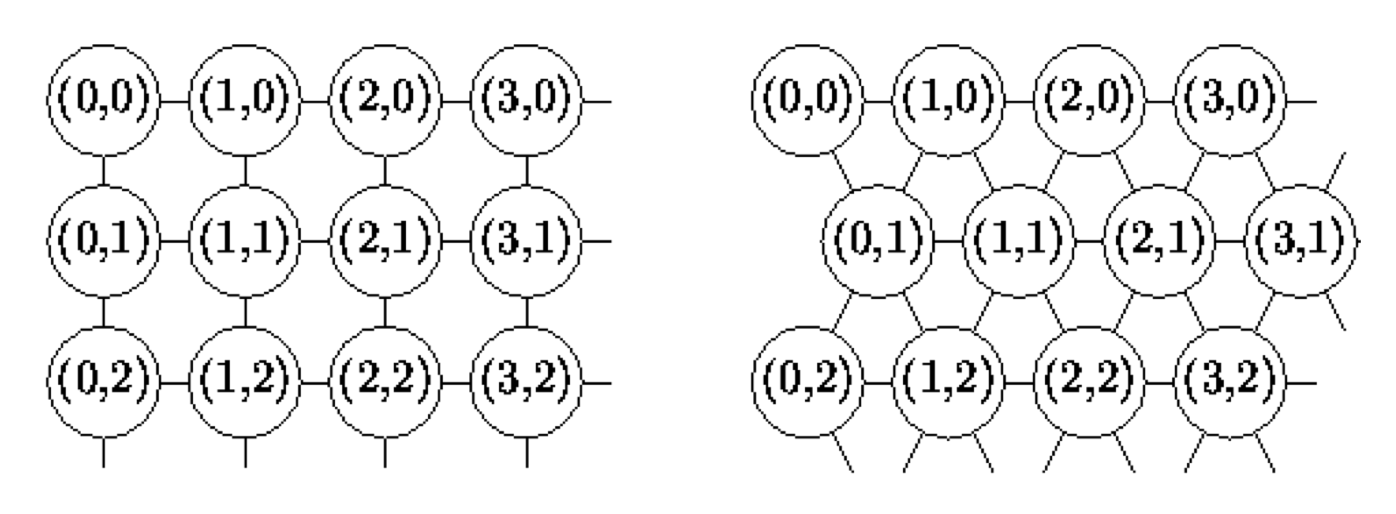
\includegraphics[scale=0.3]{lattice-structure}
	\end{center}
	For rectangular lattice Kohonen suggests the $(x,y)$ should be the ratio of the two largest eigenvalues of the autocorrelation matrix.
\end{frame}
\begin{frame}{Weight initialization}
	The most common ways of initialization is:
	\begin{enumerate}
		\item \textbf{Random initialization} Slow to converge but because SOMs are fast this may not be an issue
		\item \textbf{Random sampling initialization} Take samples from the dataset.
	\end{enumerate}
	
\end{frame}
\begin{frame}{Training the model: Step 1}
	Each lattice point has two vectors: $w_i$ representing its weight and $l_j$ representing its position within the lattice.  \\~\\
	We start by picking a random point $x \in \mathbb{R}^d$ of our data. We calculate the Euclidean distance of each lattice point from that data and select the lattice point with the smallest such distance:
	\begin{align}
		c_i = \arg \min_i \| x-w_i \|
	\end{align}
	Where $c_i$ is the index of the best matching unit. 
\end{frame}
\begin{frame}{Training the model: Step 2}
	We update the weights for all the lattice points for the $k+1$-th iteration:
	\begin{align}
		w^{(k+1)}_i = w_i^{(k)} + \alpha_k\cdot \eta_{c_i,i} \cdot \left\| x-w_i^{(k)} \right\|
	\end{align}
	Note that $\alpha_k$ is the learning rate s.t.:
	\begin{align}
		\alpha_{k+1} \leq \alpha_k \\
		\sum^\infty_{k=0} \alpha_k = \infty \\
		\sum^\infty_{k=0} \alpha_k^2 \leq \infty
	\end{align}	
\end{frame}
\begin{frame}{Training the model: Step 2}
	Note that $\eta_{c_i,i}$ is a neighborhood function, designed to: 
	\begin{enumerate}
		\item Achieve a maximum when $\|l_i-l_j \| =0$
		\item $\eta_{c_i,i} \rightarrow 0$ as $\| l_i-l_j\| \rightarrow \infty$
	\end{enumerate}
	
	
	The most common is Gaussian neighborhood:
	\begin{align}
		\eta_{c_i,i} = \exp \left[ -\frac{\|l_i - l_{c_i}\|}{2\sigma_k^2}\right]
	\end{align}
\end{frame}
\begin{frame}{Error metrics}
	Most common is quantization error:
	Let $c = \arg\min_i \|x-w_i \|$. The quantization error is then:
	\begin{align}
		E_Q = \sum_i \| x_i -w_c\|
	\end{align}
	The topographic error preserves the underlying topology of the data defined as:
	\begin{align}
		E_T = \frac{1}{|D|} \sum_{x\in D} te(x)
	\end{align}
	where:
	\begin{align}
		te(x) = \begin{cases}
			1 & \text{$c_1$ and $c_2$ are neighbors}\\
			0 & \text{else}
		\end{cases}
	\end{align}
\end{frame}
\begin{frame}{The dataset}
	We look at ride-share pickups (Uber and Lyft) for the city of Chicago in the year 20202. \\~\\
	We collate the data by census tracts, and merge the data with demographics (median income) and built-environment characteristics (percentage of zero car ownerships, distance to nearest transit) from the EPA smart locations dataset. 
\end{frame}
\section{The dataset}
\begin{frame}{The variables}
	Our variables are as follows:
	\begin{center}
	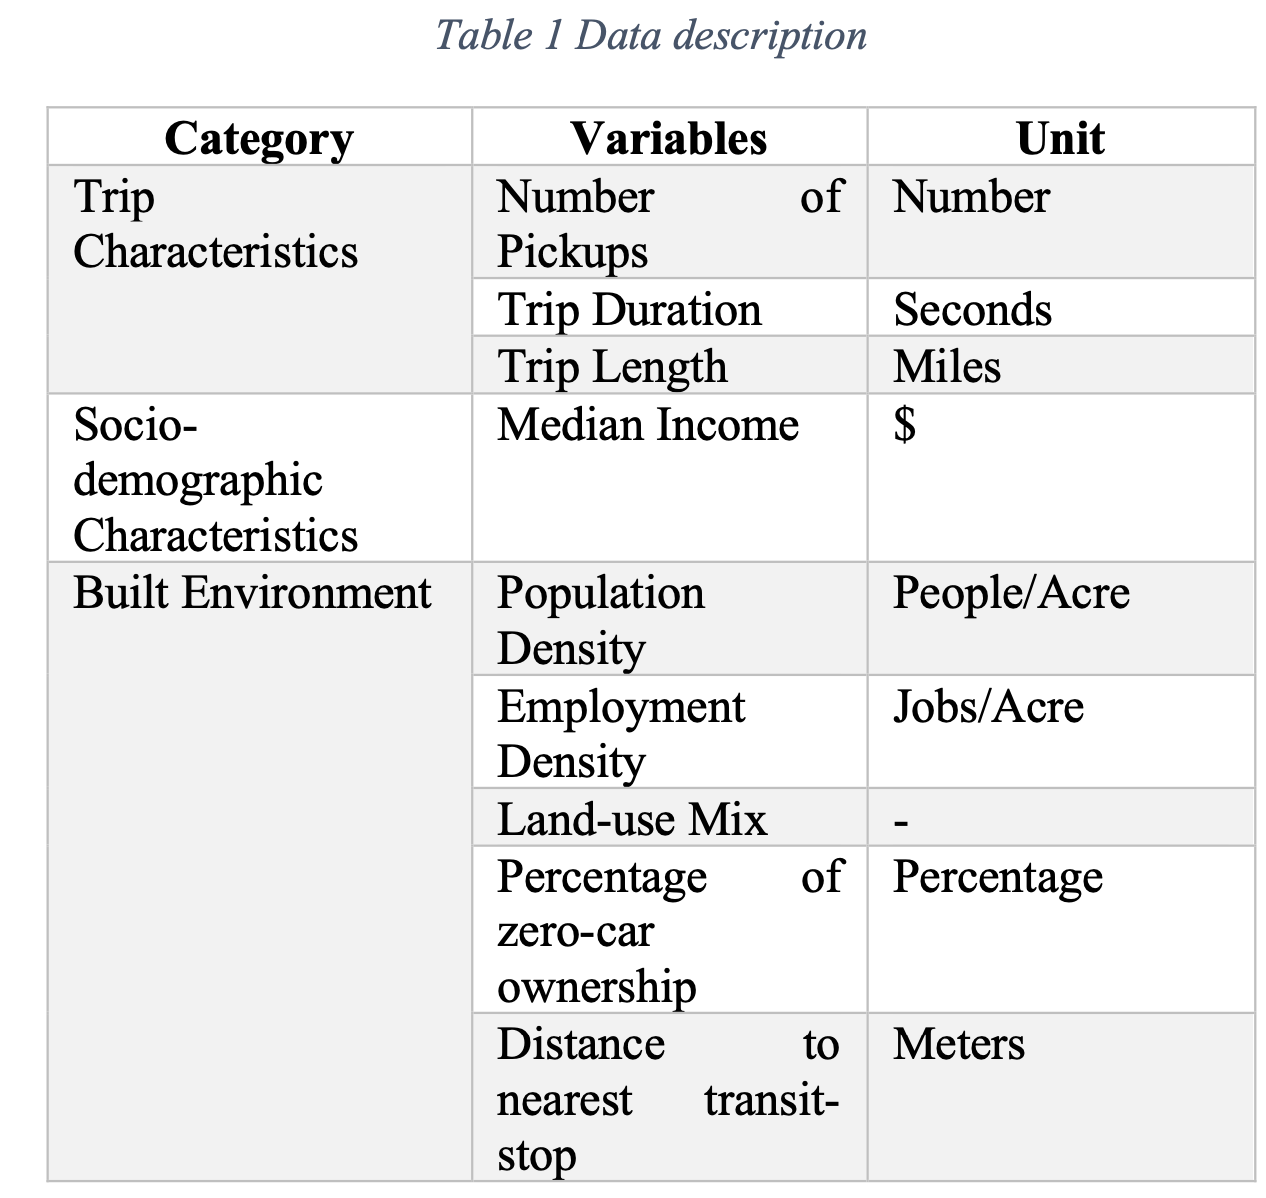
\includegraphics[scale=0.3]{variables.png}
	\end{center}
\end{frame}
\begin{frame}{Preliminary analysis}
	Previous work by the author suggests that much can be gained by doing a segmentation analysis of the dataset. \\~\\
	A principal component analysis of the scaled data shows that there exists an eigenvalue in one direction wit both components accounting for $\approx 50\%$ of the variance
	\begin{center}
	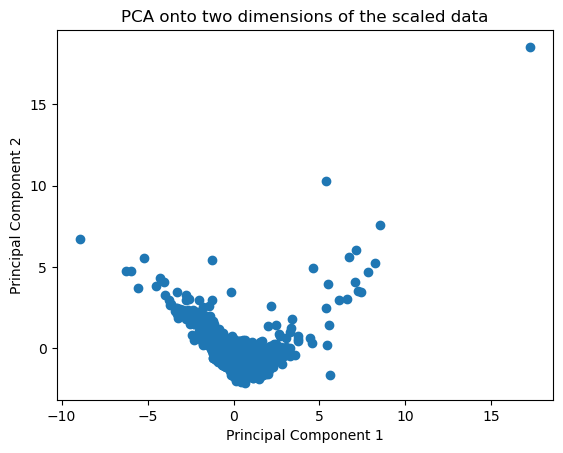
\includegraphics[scale=0.45]{pca-w.png}
	\end{center}
\end{frame}
\begin{frame}{The SOM}
	Taking a cue from previoous work we do create a $2 \times 2$ lattice. \\~\\
	Quantization errors across iteration counts shows $~600$ iterations to be optimal
	\begin{center}
		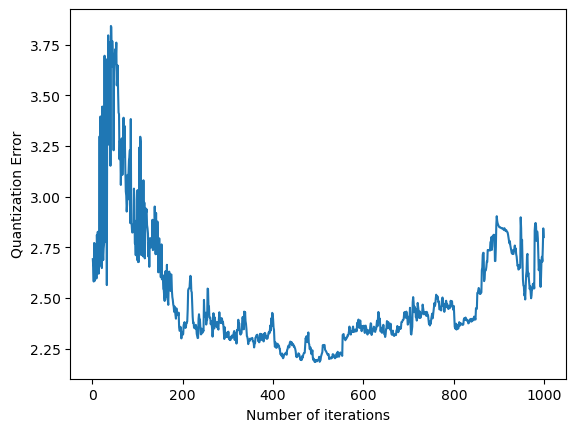
\includegraphics[scale=0.45]{quantization-error-w.png}
	\end{center}
\end{frame}
\begin{frame}{The Clustering}
	We get a clustering as such:
	\begin{center}
	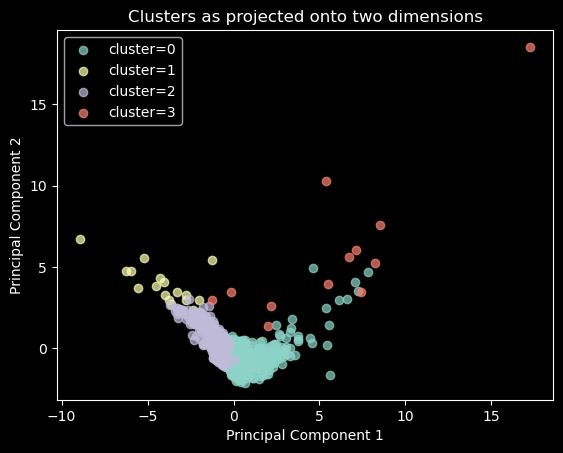
\includegraphics[scale=0.55]{cluster-pca.png}
	\end{center}
\end{frame}
\section{The results}
\begin{frame}{The Clusters I}

\begin{table}[]
\begin{tabular}{@{}llllll@{}}
\toprule
Cluster & MedIncome & PopDensity & EmpDensity & LUDiversity & \% 0 Car\\ \midrule
0 & \$85.9k & 38.18 & 10.2  & 0.82 & 24\% \\
1 & \$149k  & 10.27 & 10.46 & 3.17 & 10\% \\
2 & \$73k   & 18.32 & 3.41  & 1.01 & 14\% \\
3 & \$164k  & 31.01 & 258.6 & 45.5 & 19\% \\ \bottomrule
\end{tabular}
\end{table}

\end{frame}
\begin{frame}{The Clusters II}
\begin{table}[]
\begin{tabular}{llll}
\hline
\multicolumn{1}{l|}{Cluster} & \multicolumn{1}{l|}{Median Income} & Trip Seconds & Trip Miles \\ \hline
0 & \$85.9k & 1000.3 & 5.8  \\
1 & \$149   & 1961   & 7.5  \\
2 & \$73    & 1249   & 8.5  \\
3 & \$164   & 951    & 6.14 \\ \cline{1-1} \cline{3-4} 
\end{tabular}
\end{table}
\end{frame}
\begin{frame}{The map}
	\begin{center}
	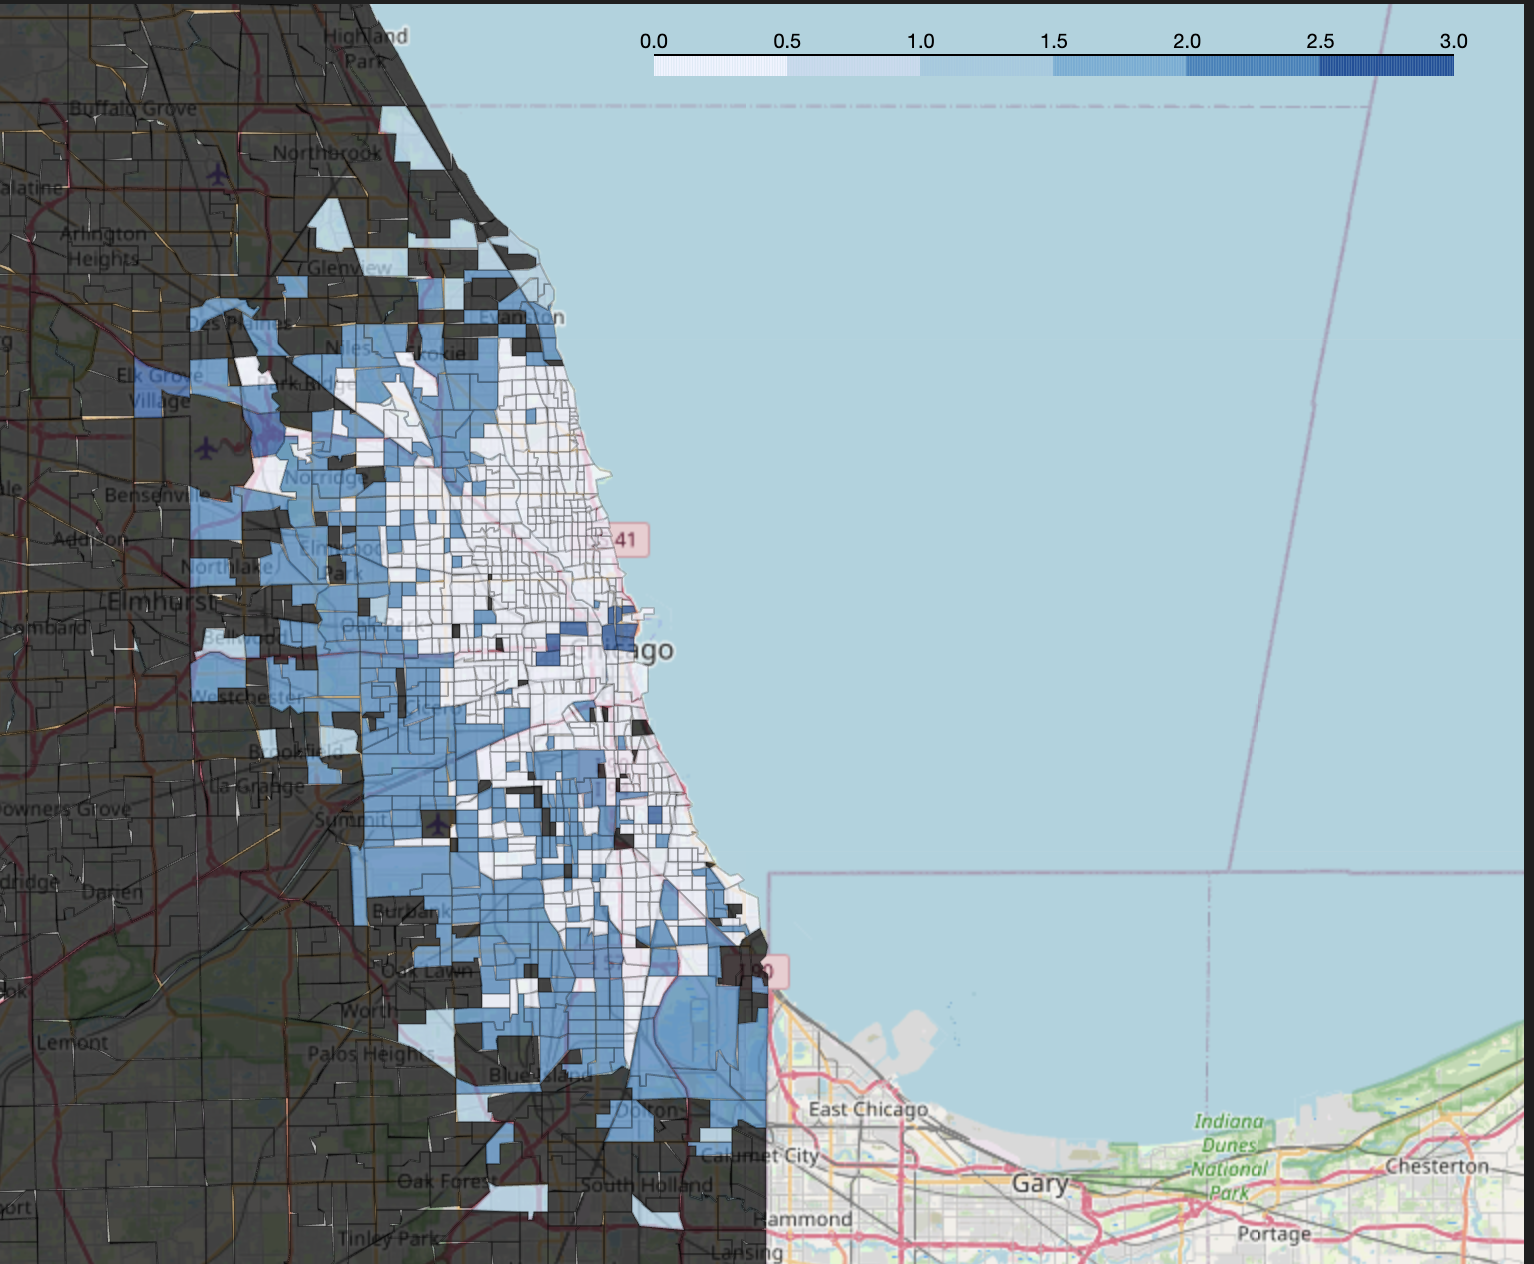
\includegraphics[scale=0.34]{map.png}
	\end{center}
\end{frame}
\begin{frame}{The Clusters III}
	The full table:
	\begin{center}
	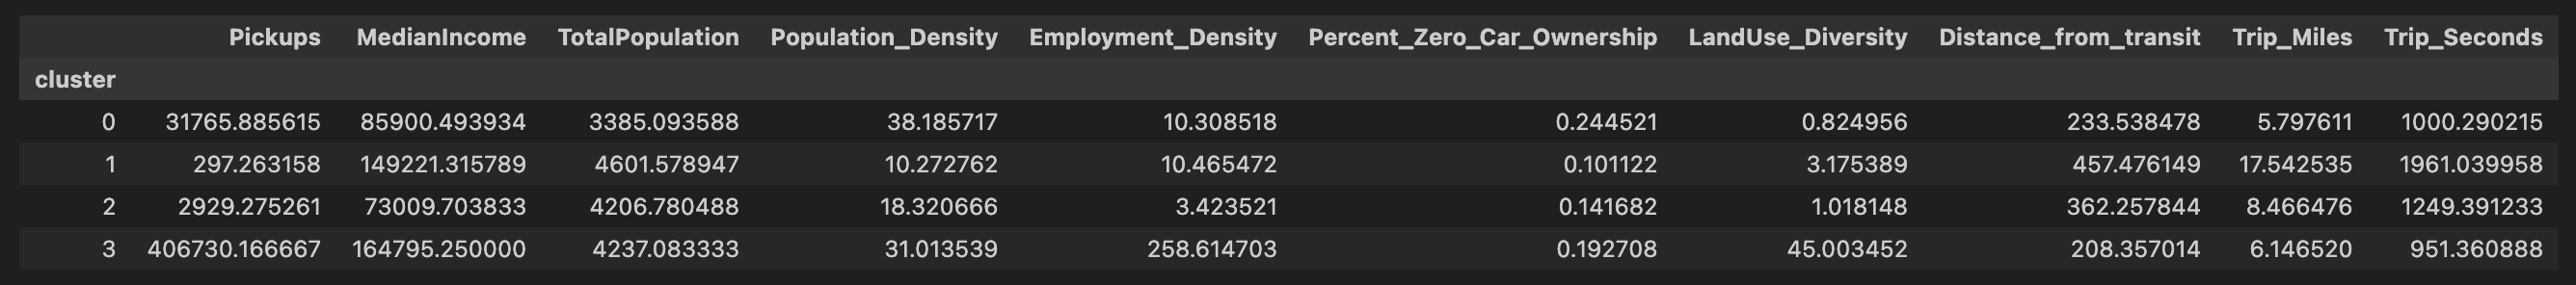
\includegraphics[scale=0.25]{full-table.png}
	\end{center}
\end{frame}
\begin{frame}{The takeaways}
	Key takeaways:
	\begin{enumerate}
		\item People from richer neighborhoods take shorter Uber trips
		\item Employment density is a better predictor than population density for the number of pickups
		\item Percentage of zero car ownership correlates with more pickups.
	\end{enumerate}
\end{frame}
\begin{frame}{Future work}
	Possible future work:
	\begin{enumerate}
		\item Could we do a detailed SHAP analysis of the factors predicting pickups, i.e. is it the case that median income of tracts can be a good predictor?
		\item Could we do a time series analysis and see a seasonality decrease around March 2020.
	\end{enumerate}
\end{frame}
\section{Future work}
\begin{frame}{Bibliography}
	\begin{enumerate}
		\item Ponmalai, Ravi, and Kamath, Chandrika. 2019. "Self-Organizing Maps and Their Applications to Data Analysis". United States. https://doi.org/10.2172/1566795. https://www.osti.gov/servlets/purl/1566795.
		\item Soria, J., Chen, Y., Stathopoulos,A., 2020. K-Prototypes Segmentation Analysis on Large-Scale Ridesourcing Trip Data, Transportation Research Board 2020, DOI: 10.1177/0361198120929338
		\item Smart Location Database. https://www.epa.gov/smartgrowth/smart- location-mapping
		\item City of Chicago Data Portal, 2021. Transportation Network Providers - Trips
	\end{enumerate}
\end{frame}
















    
    
    

    
    




\end{document}


